\documentclass{article}

\usepackage{amsmath, amssymb}
\usepackage{tikz}
\usetikzlibrary{automata, arrows.meta, positioning}
\usepackage{float}
\usepackage{caption}

\title{1DV517 - Assignment 1}
\author{Xiaoyue Chen}

\begin{document}

\maketitle

\section*{Exercise 1}
\begin{enumerate}
	\item \begin{align*}
		      (b+c)^* ((b+c)^* a (b+c)^* a (b+c)^*)^* a (b+c)^* \\
		      + (c^* b^* a c^* b^* a)^* c^* b^*
	      \end{align*}
	\item
	      \begin{align*}
		      (a+b+c)^* a (a+b+c)^* a   \\
		      + (a+b+c)^* b (a+b+c)^* b \\
		      + (a+b+c)^* c (a+b+c)^* c
	      \end{align*}
	\item DFA
	      \begin{figure*}[h]
		      \centering
		      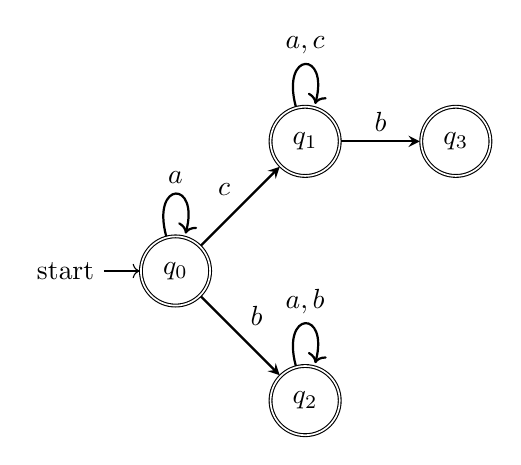
\begin{tikzpicture}[auto]
			      \node (q0) [state, initial, accepting] {$q_0$};
			      \node (q1) [state, above right = of q0, accepting] {$q_1$};
			      \node (q2) [state, below right = of q0, accepting] {$q_2$};
			      \node (q3) [state, right = of q1, accepting] {$q_3$};

			      \path [-stealth, thick]
			      (q0) edge [loop above]
			      node {$a$} ()
			      (q0) edge node {$c$} (q1)
			      (q0) edge node {$b$} (q2)
			      (q1) edge [loop above] node {$a, c$} ()
			      (q1) edge node {$b$} (q3)
			      (q2) edge [loop above] node {$a, b$} ()
			      ;
		      \end{tikzpicture}
	      \end{figure*}
\end{enumerate}

\section*{Exercise 2}
$L'$ is regular. Proof:

Since $L$ is regular, $L$ must have an
equivalent NFA. For each transition in this NFA, we remove symbols that are not
in $\Sigma'$. Now, any accepting string defined over
$\Sigma$ is projected over $\Sigma'$ because all
symbols that are not in $\Sigma'$ are removed. The resulting graph
is also an NFA. Hence the new language $L'$ is regular.

\section*{Exercise 3}
\subsection*{I}
We first show that the NFA accepts $a^+b^+$: we go from state 1
to state 2 so we have 1 $a$. To accept more
$a$s, we could loop in state 2. We then go from state 2 to
state 3 to have 1 $b$, and loop in state 3 to have more
$b$s. State 3 is an accepting state, hence the NFA accepts
$a^+b^+$.

Next we show that the NFA accepts $a^+c^*$: we go from state 1 to
state 6 to have 1 $a$, and loop in state 6 to have more
$a$s. We take the $\epsilon$ transition to state
5 if there is no $c$ in the string. If there is one or more
$c$s, we take the $c$ transition to state
5 and loop there. State 5 is an accepting state, hence the NFA accepts
$a^+c^*$.

We now show that if the previous substring is in $a^+b^+$, we
could continue to accept either $a^+b^+$ or
$a^+c^*$: if the previous substring is in $a^+b^+$,
we would be on state 3. We could take the $\epsilon$ transition to
state 1. Now, we could choose to go to either state 2 or state 6, which would
accept $a^+b^+$ or $a^+c^*$ respectively.

Finally, we show that if the previous substring is $a^+c^*$, we
could continue to accept either $a^+b^+$ or
$a^+c^*$: we are on state 5. To accept $a^+b^+$, we
could go to state 2; to accept $a^+c^*$, we could go to state 6.

Since the NFA accepts either $a^+b^+$ or $a^+c^*$,
and could continue to accept either of them indefinitely, we conclude that the
NFA accepts the language $L=(a^+b^+|a^+c^*)^+$.

\subsection*{II}
The language is $L=(ab^*a|b^+ab|b^+aab^*a)^*(ab^*|b^+a|b^+aab^*)$. Steps are shown below:

\begin{figure*}[ht]
	\caption*{Add a start and a final state}
	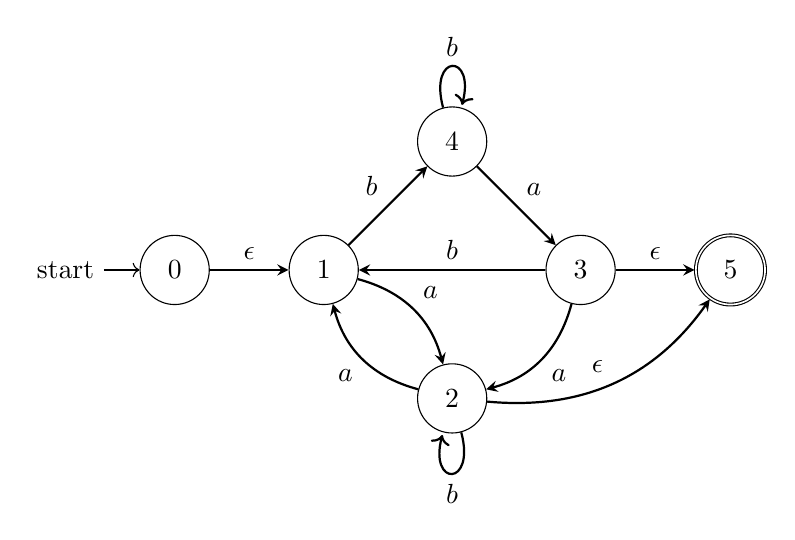
\begin{tikzpicture}[auto]
		\node (0) [state, initial] {0};
		\node (1) [state, right = of 0] {1};
		\node (2) [state, below right = of 1] {2};
		\node (3) [state, above right = of 2] {3};
		\node (4) [state, above right = of 1] {4};
		\node (5) [state, right = of 3, accepting] {5};

		\path [-stealth, thick]
		(0) edge node {$\epsilon$} (1)
		(1) edge [bend left] node {$a$} (2)
		(1) edge node {$b$} (4)
		(2) edge [loop below] node {$b$} ()
		(2) edge [bend left] node {$a$} (1)
		(2) edge [bend right] node {$\epsilon$} (5)
		(3) edge node [above] {$b$} (1)
		(3) edge [bend left] node {$a$} (2)
		(3) edge node {$\epsilon$} (5)
		(4) edge [loop above] node {$b$} ()
		(4) edge node {$a$} (3)
		;
	\end{tikzpicture}
\end{figure*}

\begin{figure*}[ht]
	\caption*{Remove state 4}
	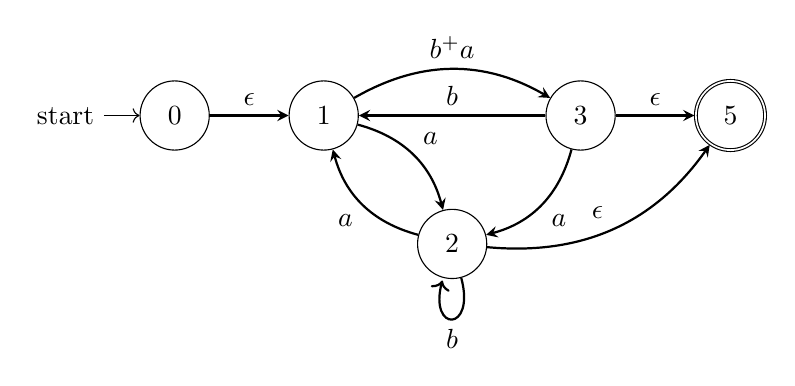
\begin{tikzpicture}[auto]
		\node (0) [state, initial] {0};
		\node (1) [state, right = of 0] {1};
		\node (2) [state, below right = of 1] {2};
		\node (3) [state, above right = of 2] {3};
		\node (5) [state, right = of 3, accepting] {5};

		\path [-stealth, thick]
		(0) edge node {$\epsilon$} (1)
		(1) edge [bend left] node {$a$} (2)
		(1) edge [bend left] node {$b^+a$} (3)
		(2) edge [loop below] node {$b$} ()
		(2) edge [bend left] node {$a$} (1)
		(2) edge [bend right] node {$\epsilon$} (5)
		(3) edge node [above] {$b$} (1)
		(3) edge [bend left] node {$a$} (2)
		(3) edge node {$\epsilon$} (5)
		;
	\end{tikzpicture}
\end{figure*}

\begin{figure*}[ht]
	\caption*{Remove state 2}
	\begin{tikzpicture}[auto]
		\node (0) [state, initial] {0};
		\node (1) [state, right = of 0] {1};
		\node (3) [state, above right = of 2] {3};
		\node (5) [state, right = of 3, accepting] {5};

		\path [-stealth, thick]
		(0) edge node {$\epsilon$} (1)
		(1) edge [loop above] node {$ab^*a$} ()
		(1) edge [bend left] node {$b^+a$} (3)
		(1) edge [bend right] node {$ab^*$} (5)
		(3) edge node {$b|ab^*a$} (1)
		(3) edge node {$\epsilon|ab^*$} (5)
		;
	\end{tikzpicture}
\end{figure*}

\begin{figure*}[ht]
	\caption*{Remove state 3}
	\begin{tikzpicture}[auto]
		\node (0) [state, initial] {0};
		\node (1) [state, right = of 0] {1};
		\node (5) [state, right = of 3, accepting] {5};

		\path [-stealth, thick]
		(0) edge node {$\epsilon$} (1)
		(1) edge [loop above] node {$ab^*a|b^+ab|b^+aab^*a$} ()
		(1) edge node {$ab^*|b^+a|b^+aab^*$} (5)
		;
	\end{tikzpicture}
\end{figure*}

\begin{figure*}[ht]
	\caption*{Remove state 1}
	\begin{tikzpicture}[auto]
		\node (0) [state, initial] {0};
		\node (5) [state, right = of 3, accepting] {5};

		\path [-stealth, thick]
		(0) edge node {$(ab^*a|b^+ab|b^+aab^*a)^*(ab^*|b^+a|b^+aab^*)$} (5)
		;
	\end{tikzpicture}
\end{figure*}

\end{document}
